% Options for packages loaded elsewhere
\PassOptionsToPackage{unicode}{hyperref}
\PassOptionsToPackage{hyphens}{url}
\documentclass[
  ignorenonframetext,
]{beamer}
\newif\ifbibliography
\usepackage{pgfpages}
\setbeamertemplate{caption}[numbered]
\setbeamertemplate{caption label separator}{: }
\setbeamercolor{caption name}{fg=normal text.fg}
\beamertemplatenavigationsymbolsempty
% remove section numbering
\setbeamertemplate{part page}{
  \centering
  \begin{beamercolorbox}[sep=16pt,center]{part title}
    \usebeamerfont{part title}\insertpart\par
  \end{beamercolorbox}
}
\setbeamertemplate{section page}{
  \centering
  \begin{beamercolorbox}[sep=12pt,center]{section title}
    \usebeamerfont{section title}\insertsection\par
  \end{beamercolorbox}
}
\setbeamertemplate{subsection page}{
  \centering
  \begin{beamercolorbox}[sep=8pt,center]{subsection title}
    \usebeamerfont{subsection title}\insertsubsection\par
  \end{beamercolorbox}
}
% Prevent slide breaks in the middle of a paragraph
\widowpenalties 1 10000
\raggedbottom
\AtBeginPart{
  \frame{\partpage}
}
\AtBeginSection{
  \ifbibliography
  \else
    \frame{\sectionpage}
  \fi
}
\AtBeginSubsection{
  \frame{\subsectionpage}
}
\usepackage{iftex}
\ifPDFTeX
  \usepackage[T1]{fontenc}
  \usepackage[utf8]{inputenc}
  \usepackage{textcomp} % provide euro and other symbols
\else % if luatex or xetex
  \usepackage{unicode-math} % this also loads fontspec
  \defaultfontfeatures{Scale=MatchLowercase}
  \defaultfontfeatures[\rmfamily]{Ligatures=TeX,Scale=1}
\fi
\usepackage{lmodern}
\ifPDFTeX\else
  % xetex/luatex font selection
\fi
% Use upquote if available, for straight quotes in verbatim environments
\IfFileExists{upquote.sty}{\usepackage{upquote}}{}
\IfFileExists{microtype.sty}{% use microtype if available
  \usepackage[]{microtype}
  \UseMicrotypeSet[protrusion]{basicmath} % disable protrusion for tt fonts
}{}
\makeatletter
\@ifundefined{KOMAClassName}{% if non-KOMA class
  \IfFileExists{parskip.sty}{%
    \usepackage{parskip}
  }{% else
    \setlength{\parindent}{0pt}
    \setlength{\parskip}{6pt plus 2pt minus 1pt}}
}{% if KOMA class
  \KOMAoptions{parskip=half}}
\makeatother
\usepackage{graphicx}
\makeatletter
\newsavebox\pandoc@box
\newcommand*\pandocbounded[1]{% scales image to fit in text height/width
  \sbox\pandoc@box{#1}%
  \Gscale@div\@tempa{\textheight}{\dimexpr\ht\pandoc@box+\dp\pandoc@box\relax}%
  \Gscale@div\@tempb{\linewidth}{\wd\pandoc@box}%
  \ifdim\@tempb\p@<\@tempa\p@\let\@tempa\@tempb\fi% select the smaller of both
  \ifdim\@tempa\p@<\p@\scalebox{\@tempa}{\usebox\pandoc@box}%
  \else\usebox{\pandoc@box}%
  \fi%
}
% Set default figure placement to htbp
\def\fps@figure{htbp}
\makeatother
\setlength{\emergencystretch}{3em} % prevent overfull lines
\providecommand{\tightlist}{%
  \setlength{\itemsep}{0pt}\setlength{\parskip}{0pt}}
% Auto-generated by infrastructure/rendering/_pdf_latex_helpers.py::extract_math_font_preamble.
% Minimal header passed to Pandoc via -H so Beamer slides pick up the same math font
% as the combined-PDF path. Adjust the manuscript's preamble.md to change the font globally.
\usepackage{unicode-math}
\setmathfont{latinmodern-math.otf}
\usepackage{bookmark}
\IfFileExists{xurl.sty}{\usepackage{xurl}}{} % add URL line breaks if available
\urlstyle{same}
\hypersetup{
  hidelinks,
  pdfcreator={LaTeX via pandoc}}

\author{\texorpdfstring{}{}}
\date{}

\begin{document}

\section{Compact Closure: Snake Equation, Valency, and Four Complexity
Metrics}\label{sec:compact-closure-complexity}

\begin{frame}[allowframebreaks]{Compact Closure: Snake Equation,
Valency, and Four Complexity Metrics}
\textbf{Where we are in the argument.}
\autoref{sec:categorial-grammar}--\autoref{sec:categorical-semantics}
made each sentence a string diagram that simultaneously expresses syntax
and semantics. This chapter zooms in on the \emph{axiom} that makes the
machine run --- the compact-closure snake equation
\((\varepsilon_n \otimes 1_n) \circ (1_n \otimes \eta_n) = 1_n\) --- and
uses its consequences to define four graded complexity metrics (word
count, cup count, cap count, depth) that turn ``how hard is this
sentence to parse?'' from a qualitative question into a computable one,
feeding directly into the enriched hom-values of
\autoref{sec:enriched-categories}.
\end{frame}

\begin{frame}[fragile,allowframebreaks]{The Snake Equation Powers Every
Pregroup Contraction}
\protect\phantomsection\label{the-snake-equation-powers-every-pregroup-contraction}
\begin{block}{The Snake Equation (Zigzag Identity)}
\protect\phantomsection\label{the-snake-equation-zigzag-identity}
The essential algebraic engine driving DisCoCat is the strict
\textbf{compact closure} of the governing pregroup category. For every
lexical type \(n\), the corresponding adjunction
maps---\(\eta_n: 1 \to n \otimes n^r\) (the cap expansion) and
\(\varepsilon_n: n^r \otimes n \to 1\) (the cup contraction)---must
mathematically satisfy the fundamental \textbf{snake equation} (also
known as the topological zigzag identity):

\begin{equation}
(\varepsilon_n \otimes 1_n) \circ (1_n \otimes \eta_n) = 1_n
\label{eq:eq-4-3}
\end{equation}

Translated into intuitive string-diagrammatic terms, a cup geometrically
composed with a cap bridging adjacent wires immediately ``straightens
out'' into a solid identity wire---a topological zigzag seamlessly
canceling into a continuous straight line. This foundational axiom is
not merely a geometric curiosity: it physically functions as the
\emph{engine} powering every valid pregroup type reduction. Every
recorded grammatical contraction (e.g., a noun canceling against an
active verb argument slot) constitutes a direct instance of the cup map
\(\varepsilon{}\), and every grammatical expansion instantiates the cap
map \(\eta{}\). The continuous snake equation algebraically guarantees
that these interwoven contractions and expansions remain globally
well-behaved---ensuring they can be freely inserted and removed without
ever altering the final semantic meaning of the derivation.

Cognitively, the snake equation provides an immediate \emph{visual
proof} of coherence. A cognitive agent inspecting a string diagram can
verify well-formedness by confirming that all zigzags cancel---a purely
spatial operation requiring no sequential algebraic computation, and
thus instantiating Shimojima's {[}-@shimojima1996reasoning{]} free-ride
inference in its most direct form (\autoref{fig:discopy-snake}).

\begin{figure}
\centering
\pandocbounded{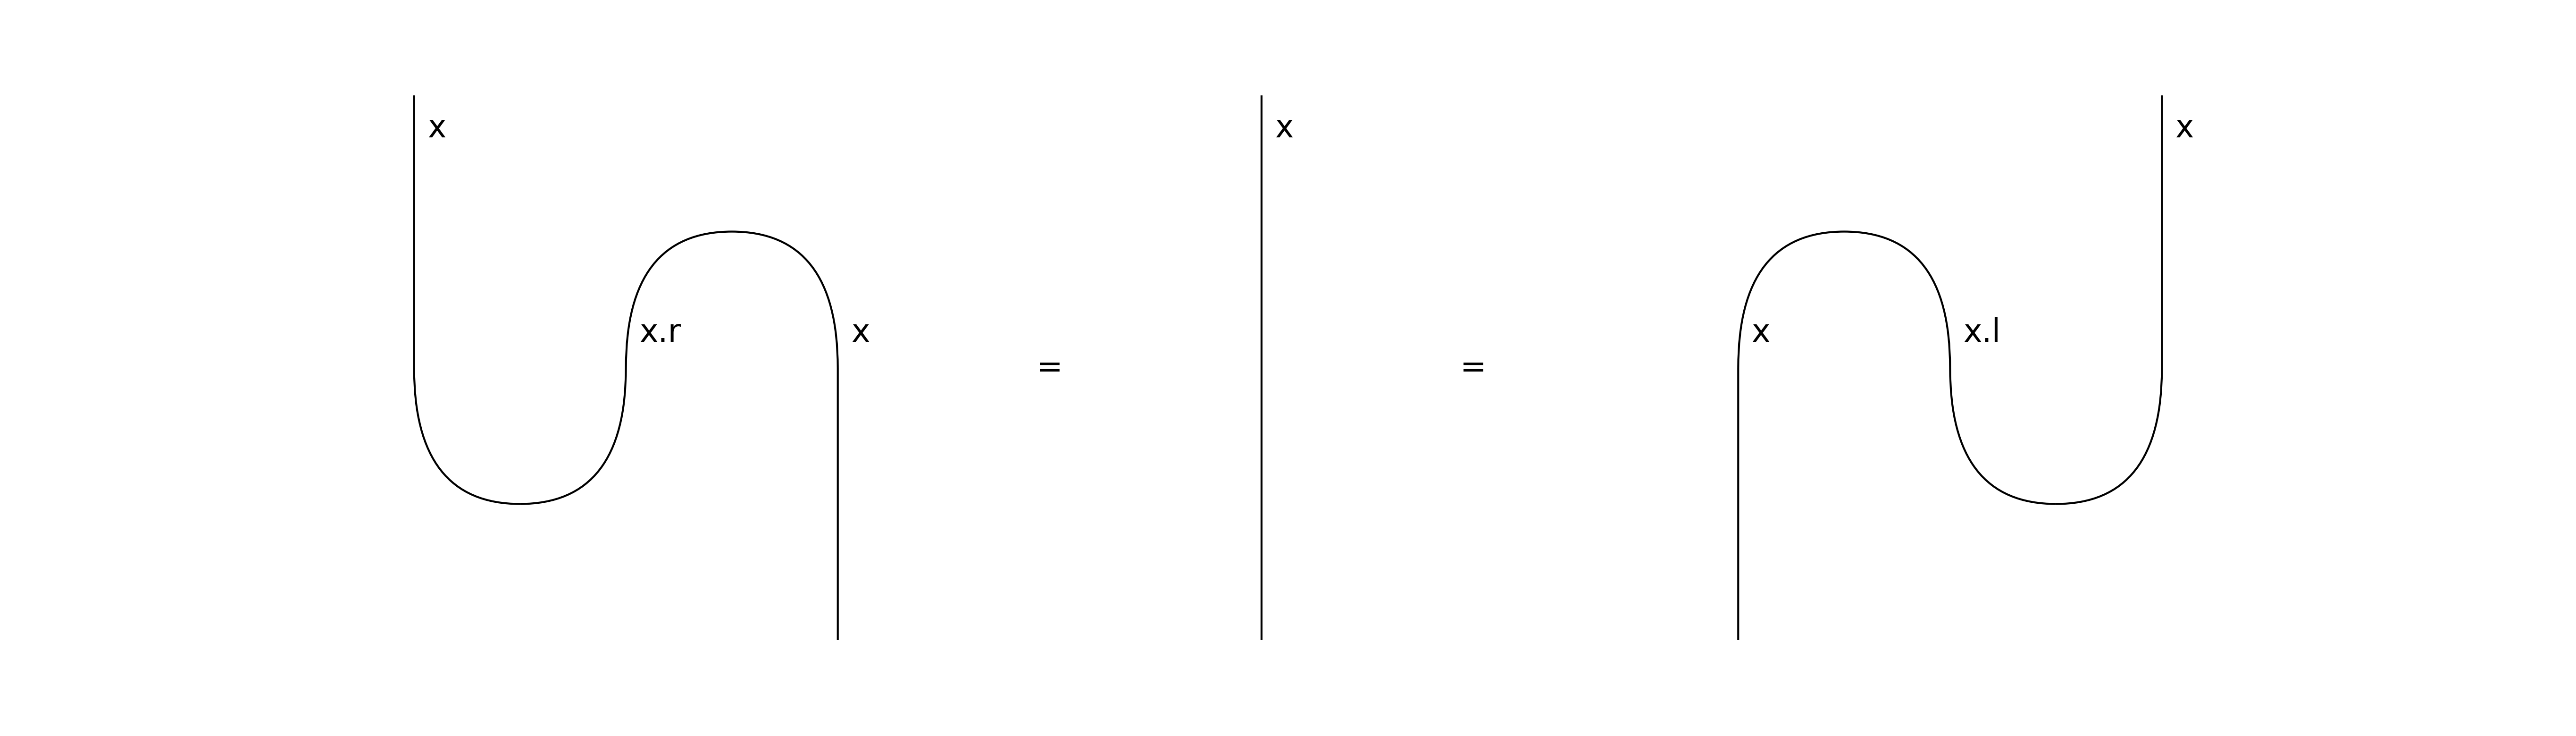
\includegraphics[keepaspectratio,alt={The snake equation is the algebraic engine powering every pregroup type reduction. The compact closure axiom () rendered by DisCoPy as a three-panel equality: left panel shows the right-adjoint zigzag (\textbackslash varepsilon\_n \textbackslash otimes 1\_n) \textbackslash circ (1\_n \textbackslash otimes \textbackslash eta\_n) with the x\^{}r intermediary; middle panel is the identity wire 1\_n that the zigzag equals; right panel shows the mirror-image left-adjoint zigzag using the x\^{}l adjoint. Verified computationally via diagram.normal\_form() == Id(Ty(\textquotesingle x\textquotesingle)). Each pregroup contraction (noun canceling with verb argument) is an instance of \textbackslash varepsilon\{\}; the snake equation guarantees that cup-cap pair insertions and removals leave derivations invariant (cf.~). Generated by render\_discopy\_snake() in src/visualization/discopy\_diagrams.py.}]{../figures/discopy_snake.png}}
\caption{The snake equation is the algebraic engine powering every
pregroup type reduction. The compact closure axiom (\autoref{eq:eq-4-3})
rendered by DisCoPy as a three-panel equality: \textbf{left panel} shows
the right-adjoint zigzag
\((\varepsilon_n \otimes 1_n) \circ (1_n \otimes \eta_n)\) with the
\(x^r\) intermediary; \textbf{middle panel} is the identity wire \(1_n\)
that the zigzag equals; \textbf{right panel} shows the mirror-image
left-adjoint zigzag using the \(x^l\) adjoint. Verified computationally
via
\protect\texttt{diagram.normal\_form()\ ==\ Id(Ty(\textquotesingle{}x\textquotesingle{}))}.
Each pregroup contraction (noun canceling with verb argument) is an
instance of \(\varepsilon{}\); the snake equation guarantees that
cup-cap pair insertions and removals leave derivations invariant
(cf.~\autoref{sec:categorial-grammar}). Generated by
\protect\texttt{render\_discopy\_snake()} in
\protect\texttt{src/visualization/discopy\_diagrams.py}.}\label{fig:discopy-snake}
\end{figure}

\autoref{fig:snake-unpacking} unpacks the same axiom into three explicit
panels: the left-hand zigzag carrying its \(\eta_n\) and
\(\varepsilon_n\) labels, the identity wire \(1_n\) it equals, and an
algebraic recap of both compact-closure equations with cap and cup type
signatures.

\begin{figure}
\centering
\pandocbounded{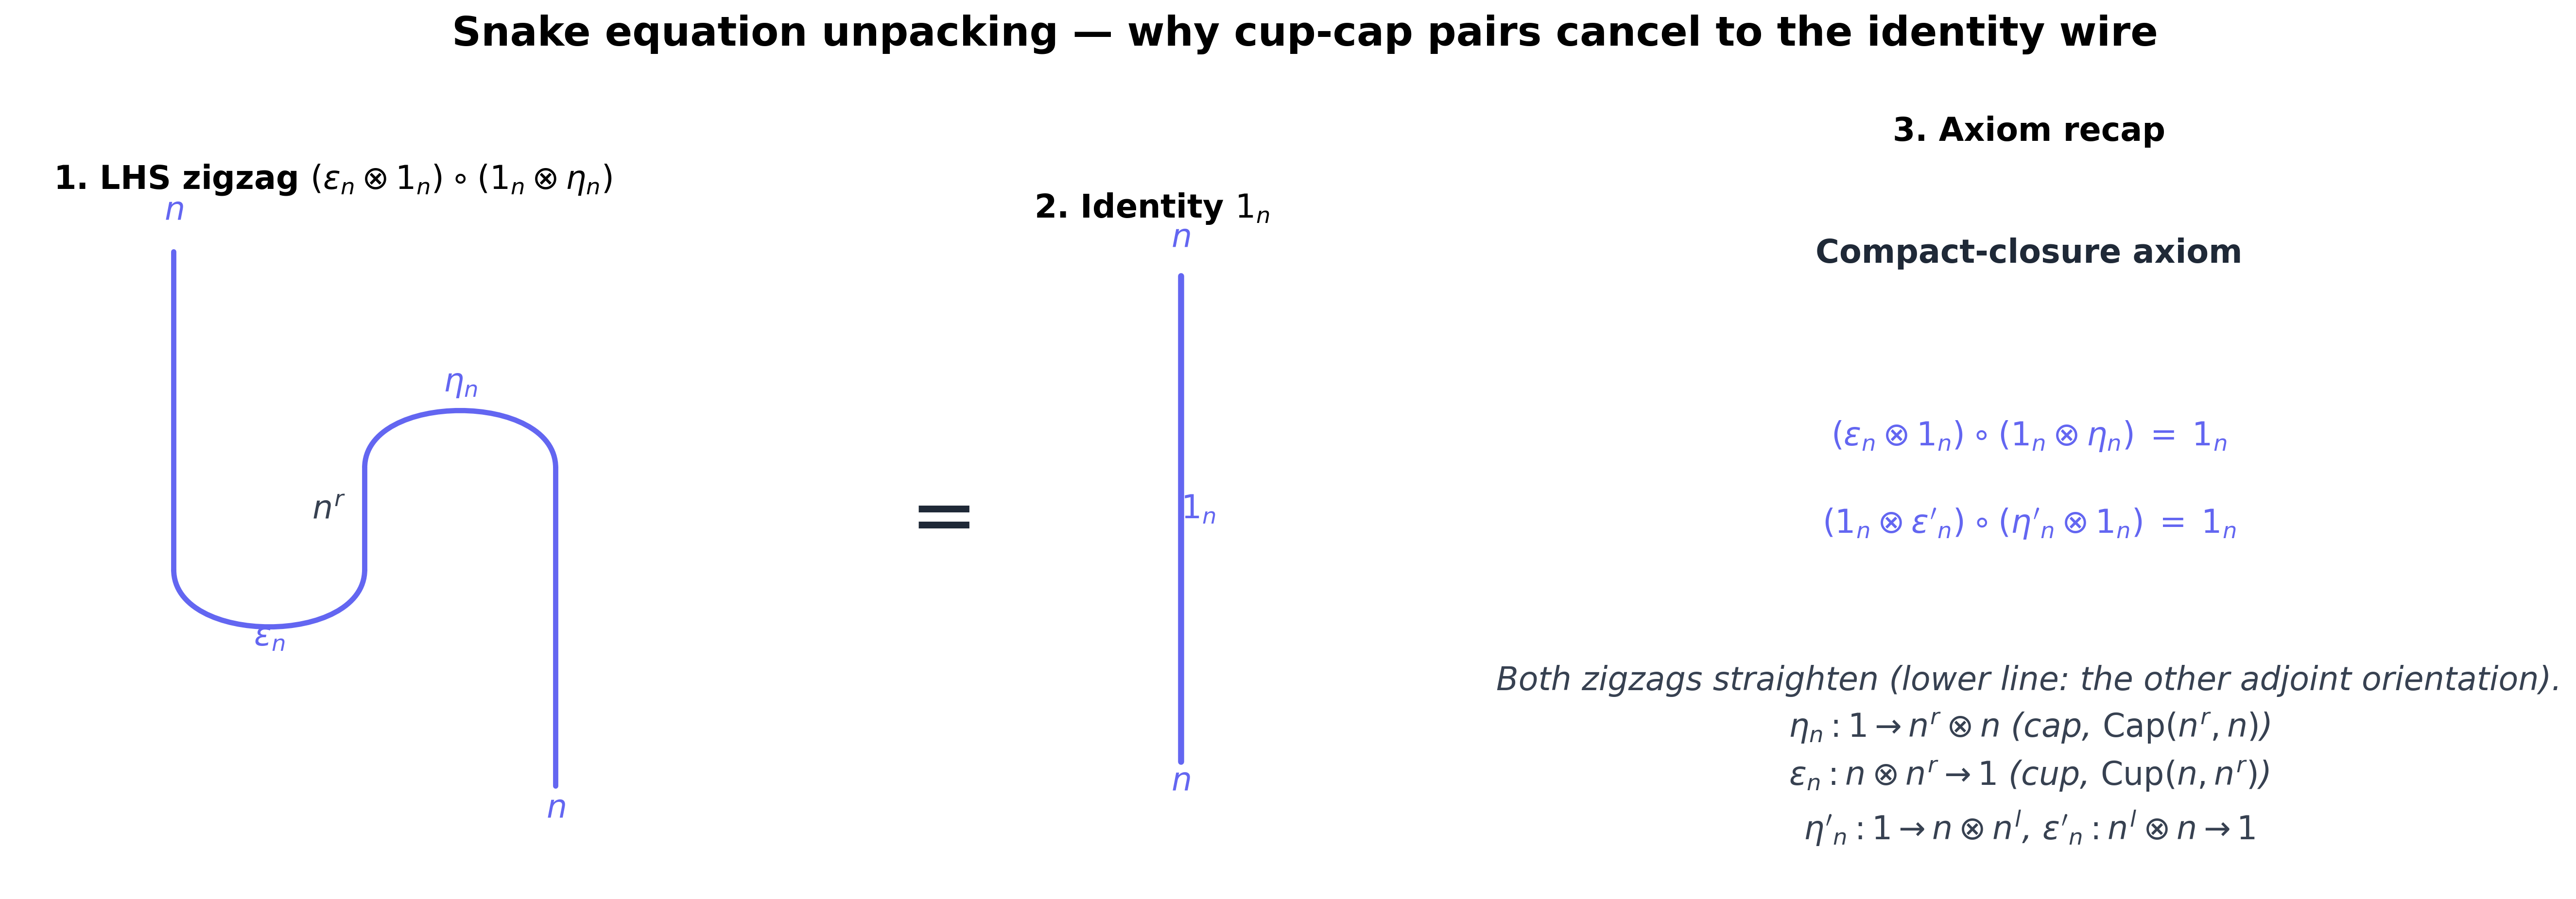
\includegraphics[keepaspectratio,alt={Snake equation unpacked. Panel 1: the zigzag (\textbackslash varepsilon\_n \textbackslash otimes 1\_n) \textbackslash circ (1\_n \textbackslash otimes \textbackslash eta\_n) with η at the top (cap, 1 \textbackslash to n \textbackslash otimes n\^{}r) and ε at the bottom (cup, n\^{}r \textbackslash otimes n \textbackslash to 1). Panel 2: the identity wire 1\_n it equals. Panel 3: axiom recap showing both zigzag equations straighten to the identity, with explicit type signatures for η and ε. Generated programmatically from src.visualization.category\_unpacking.render\_snake\_equation\_unpacking().}]{../figures/snake_equation_unpacking.png}}
\caption{Snake equation unpacked. Panel 1: the zigzag
\((\varepsilon_n \otimes 1_n) \circ (1_n \otimes \eta_n)\) with η at the
top (cap, \(1 \to n \otimes n^r\)) and ε at the bottom (cup,
\(n^r \otimes n \to 1\)). Panel 2: the identity wire \(1_n\) it equals.
Panel 3: axiom recap showing both zigzag equations straighten to the
identity, with explicit type signatures for η and ε. Generated
programmatically from
\protect\texttt{src.visualization.category\_unpacking.render\_snake\_equation\_unpacking()}.}\label{fig:snake-unpacking}
\end{figure}
\end{block}

\begin{block}{Four Metrics Quantify Derivational Complexity}
\protect\phantomsection\label{four-metrics-quantify-derivational-complexity}
The algebraic properties of pregroup diagrams support quantitative
analysis of derivational complexity. Our \texttt{complexity\_metrics}
module implements four complementary measures using the DisCoPy library:

\begin{enumerate}
\item
  \textbf{Box count}: The number of lexical entries (Word boxes) in the
  diagram, corresponding to the sentence's word count from the
  type-logical perspective. A transitive sentence has 3 boxes (subject,
  verb, object); a ditransitive sentence has 4 or more.
\item
  \textbf{Cup/Cap count}: The number of contraction and expansion
  operations. Cups (denoted \(\varepsilon{}\)) count argument
  consumption; caps (denoted \(\eta{}\)) count argument introduction.
  The cup count directly reflects verb valency: an intransitive verb
  requires 1 cup, a transitive verb 2, and a ditransitive verb 3.
\item
  \textbf{Normal form}: A diagram is in \emph{normal form} if no further
  simplifications (zigzag cancellations, box reordering) are possible.
  The \texttt{compute\_normal\_form()} operation computes this canonical
  representative of the diagram's equivalence class. Normal form
  preservation under algebraic manipulation provides a correctness check
  for compositional operations.
\item
  \textbf{Syntactic complexity score}: A composite metric defined as:
\end{enumerate}

\begin{equation}
\text{complexity}(D) = w_w \cdot |D|_{\text{words}} + w_c \cdot |D|_{\text{cup}} + w_a \cdot |D|_{\text{cap}} + w_d \cdot \text{depth}(D)
\label{eq:eq-4-4}
\end{equation}

where \(|D|_{\text{words}}\) is the \emph{lexical} box count (Cup/Cap
plumbing excluded), \(|D|_{\text{cup}}\) and \(|D|_{\text{cap}}\) are
contraction and expansion counts, and \(\text{depth}(D)\) is the longest
input-to-output path measured in boxes. The weights
\(w_w, w_c, w_a, w_d\) are keyword arguments to
\texttt{syntactic\_complexity\_score()}; the defaults \(w_w{=}1.0\),
\(w_c{=}0.5\), \(w_a{=}0.25\), \(w_d{=}0.1\) encode the intuition that
lexical entries contribute most, contractions moderately, expansions
least, and depth a small residual penalty. Passing
\(w_w{=}w_c{=}w_a{=}w_d{=}1.0\) recovers an unweighted total-structure
count. Deeper diagrams encode more complex syntactic derivations---a
ditransitive sentence like ``Alice gave Bob a book'' (depth 7) is
structurally more complex than a simple intransitive ``Alice runs''
(depth 3).

The \texttt{compare\_diagrams()} function applies these metrics across a
collection of diagrams, producing tabular comparisons suitable for
cross-linguistic analysis. \autoref{fig:complexity-comparison}
visualizes these metrics across sentence types of increasing valency,
demonstrating the monotonic relationship between argument structure and
derivational complexity.

\begin{figure}
\centering
\pandocbounded{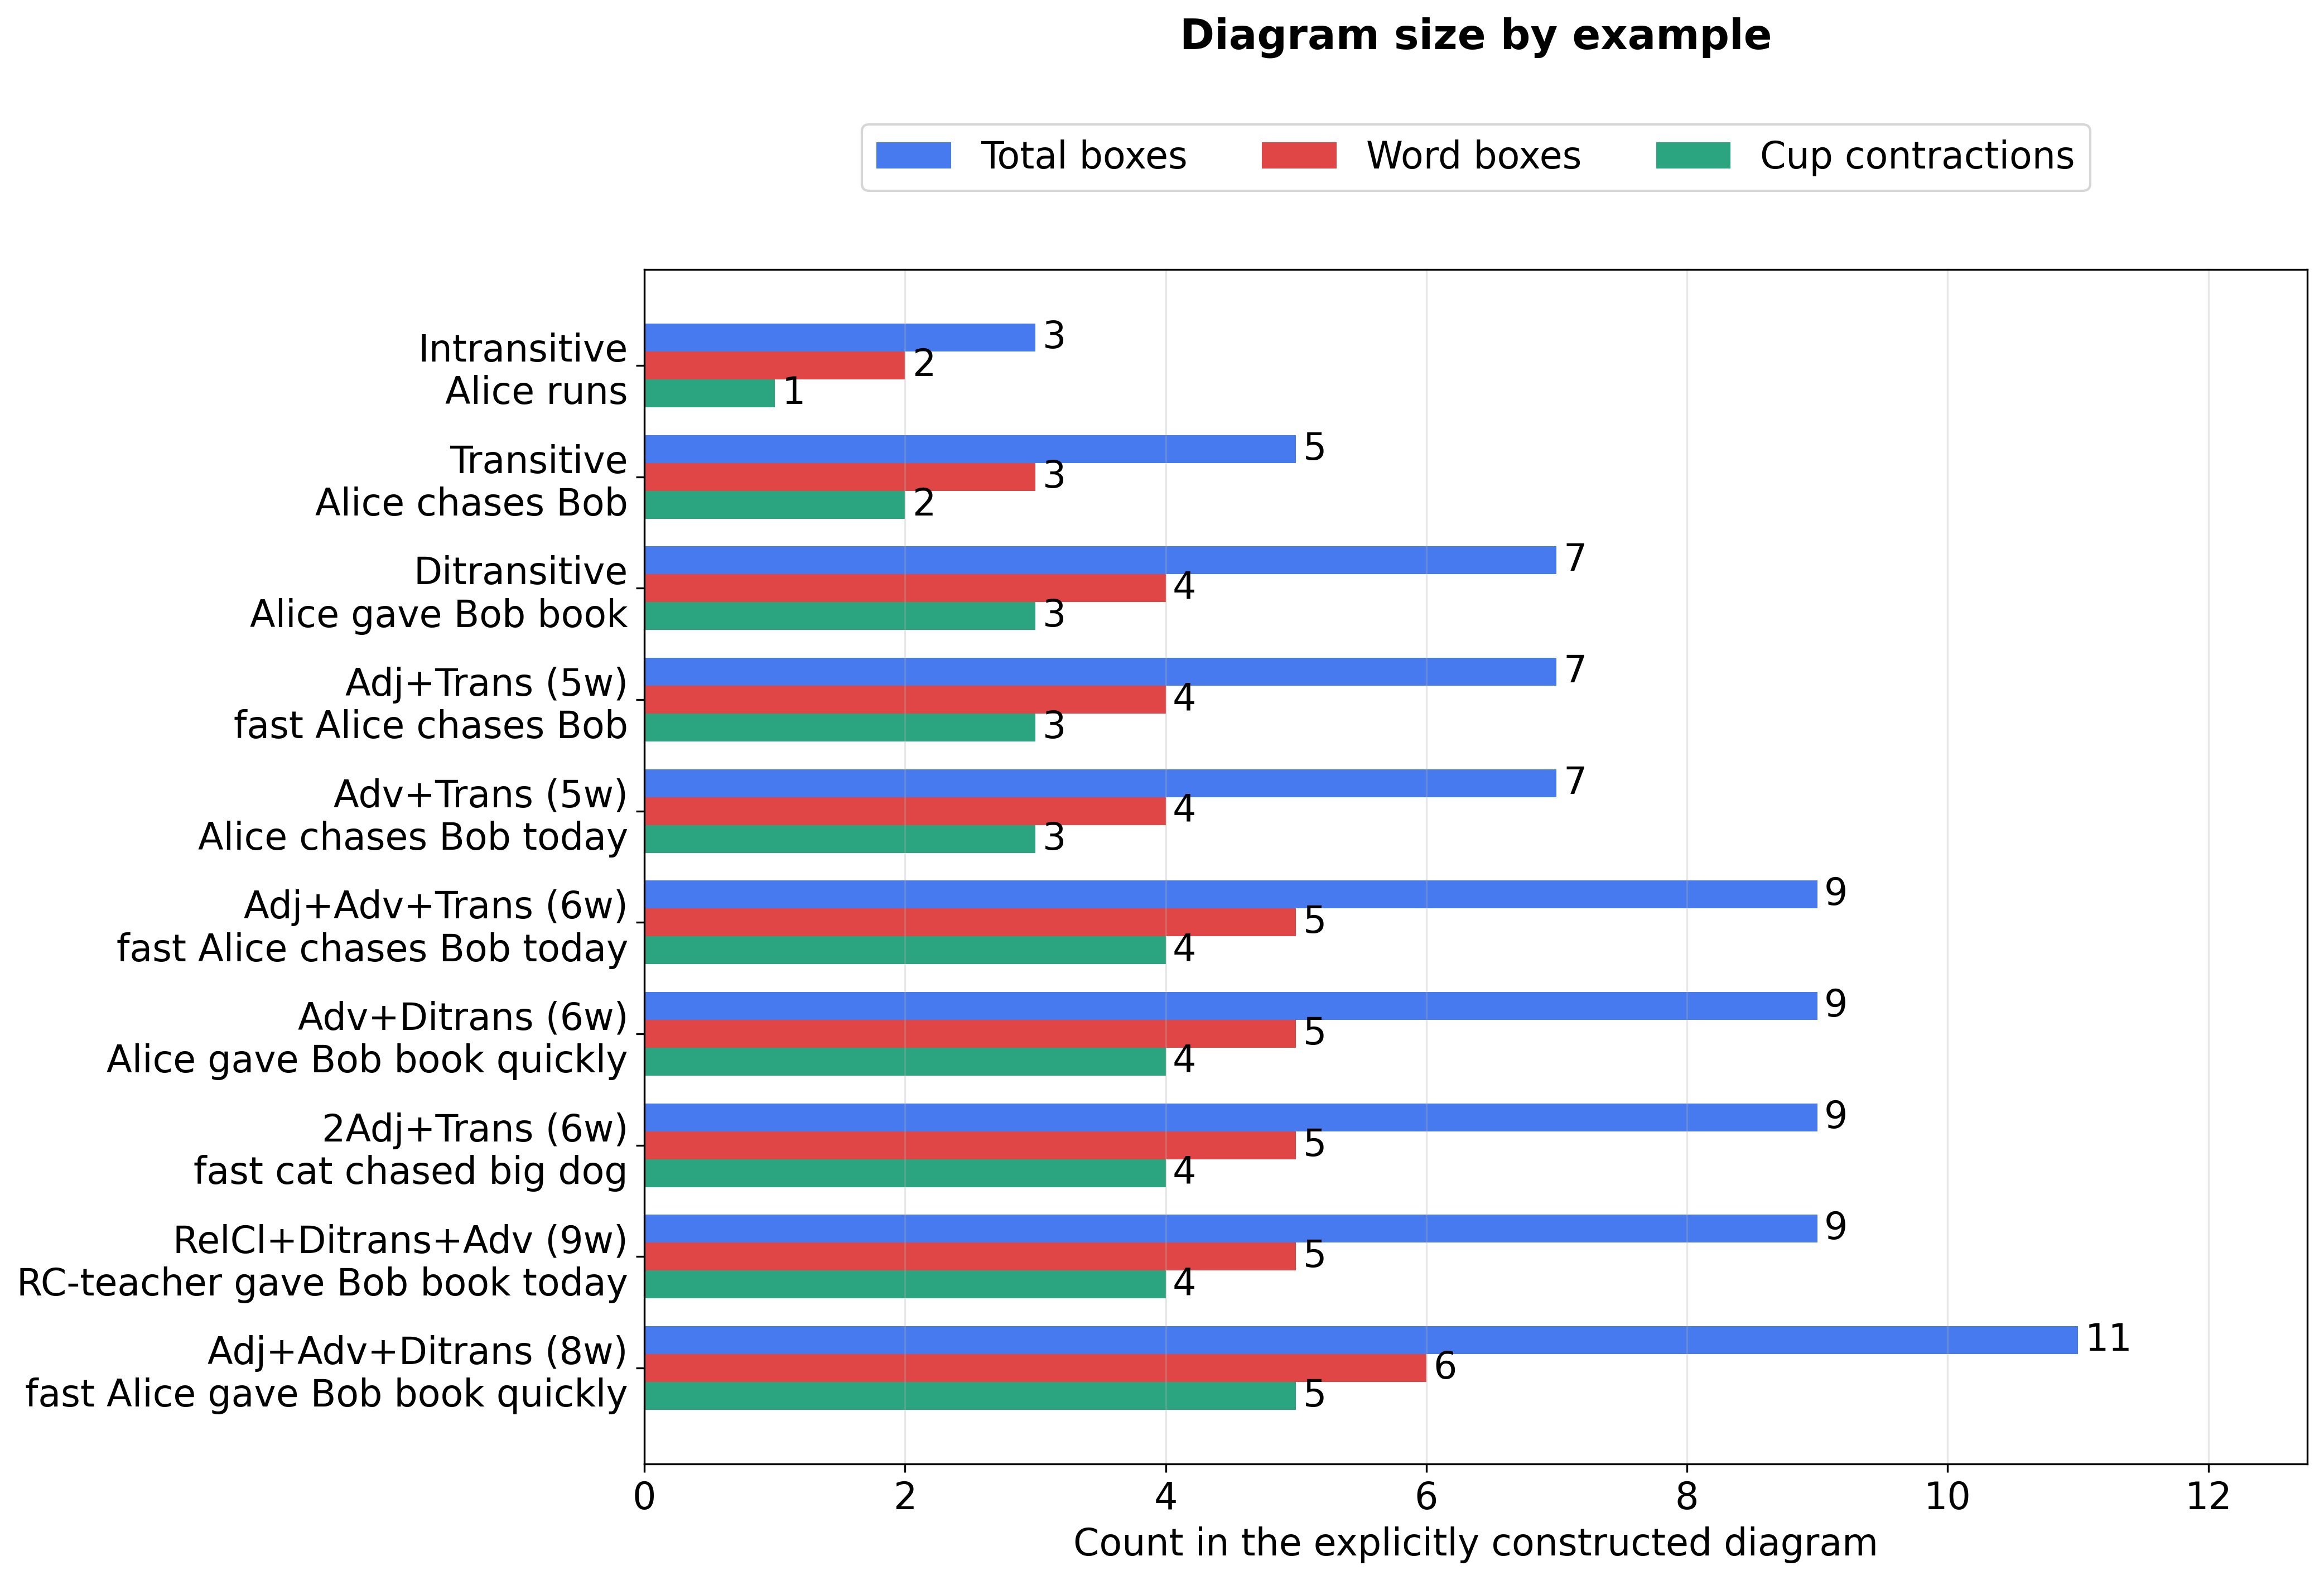
\includegraphics[keepaspectratio,alt={Verb valency dominates diagram complexity: categorical complexity score \textbackslash kappa(D) () plotted for ten sentence types ranging from intransitive to adjunct-heavy constructions, with natural-language exemplar sentences overlaid at each bar. Generated by render\_complexity\_comparison() in src/visualization/complexity\_plots.py (orchestrated by scripts/generate\_diagrams.py).}]{../figures/complexity_comparison.png}}
\caption{Verb valency dominates diagram complexity: categorical
complexity score \(\kappa(D)\) (\autoref{eq:eq-4-4}) plotted for ten
sentence types ranging from intransitive to adjunct-heavy constructions,
with natural-language exemplar sentences overlaid at each bar. Generated
by \protect\texttt{render\_complexity\_comparison()} in
\protect\texttt{src/visualization/complexity\_plots.py} (orchestrated by
\protect\texttt{scripts/generate\_diagrams.py}).}\label{fig:complexity-comparison}
\end{figure}

\textbf{Key finding.} Adverb and adjective modifiers increase box count
but do not always add core argument Cups (modifier types \(n \cdot n^l\)
contribute one box and one cup each, but some adverbs add a box without
an argument Cup), so \(\kappa{}\) can grow more slowly with adjunct
stacking than with valency increases. Cup count
\(\lvert D\rvert_{\text{cup}}\) remains a reliable proxy for verb
valency. In code, cup counts are obtained by iterating DisCoPy diagram
boxes and testing for \texttt{Cup} instances (see
\texttt{compare\_diagrams()} in the project).

These metrics connect naturally to the enriched framework of
\autoref{sec:enriched-categories}: diagram depth serves as a syntactic
complexity proxy that can be incorporated into the enriched hom-value,
providing a principled bridge between type-logical derivation cost and
distributional semantic distance. Discourse-level persistence of entity
wires (DisCoCirc) is developed in \autoref{sec:discocirc-discourse}. For
multi-agent security, when tracking networks isolate an adversarial
identity wire (a prompt injection) covertly attempting to merge with an
ongoing command wire across communication boundaries, the circuit
topology can flag the type violation before execution
(\autoref{sec:cognitive-security}).
\end{block}
\end{frame}

\end{document}
